\section{Maquettage}

Afin de réaliser l'étape la plus longue de ce lot, nous avons répertorié toutes les routes nécessaires et nous avons réalisé un diagramme nous permettant de correctement recenser toutes les pages du client.

\begin{figure}[th]
\centering
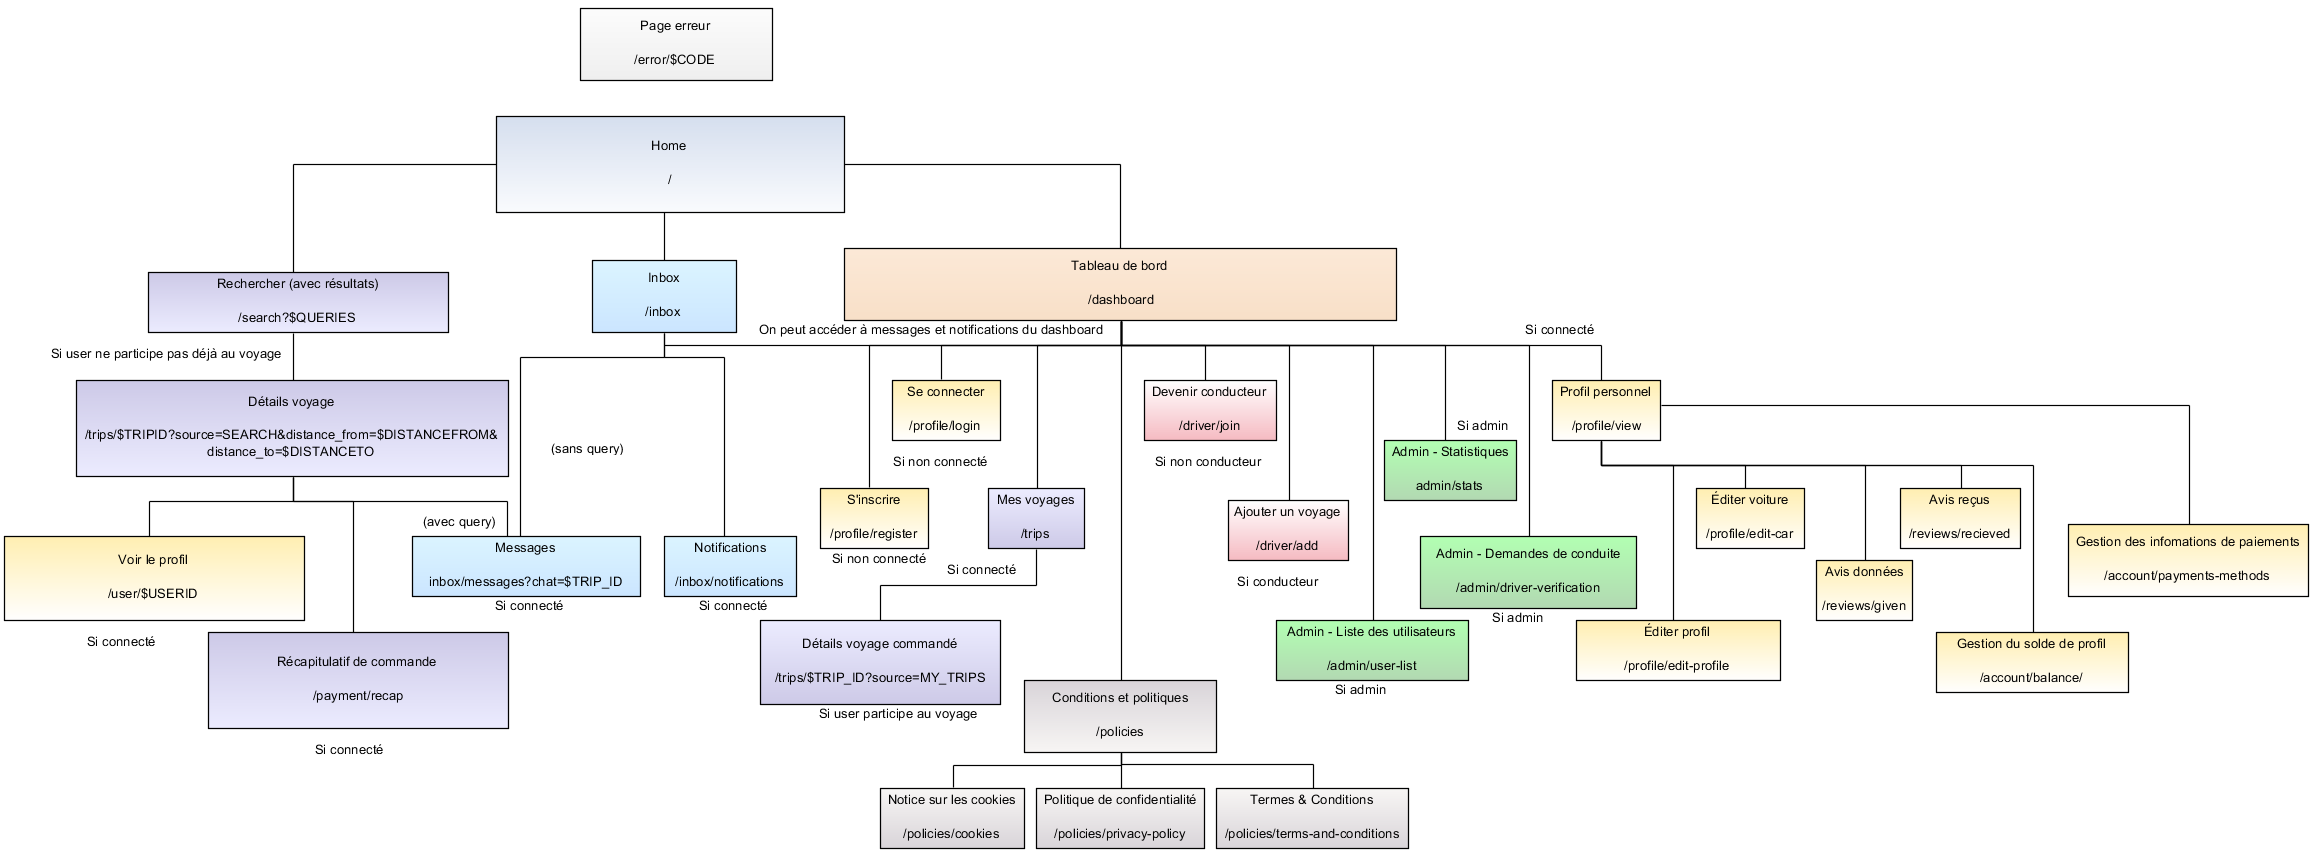
\includegraphics[width=\linewidth]{medias/sitemap.png}
\decoRule
\caption{Plan du site (voir en grand: \ref{Plan du site})}
\end{figure}

Comme indiqué précédemment, le site étant "mobile first", nous nous sommes concentrés sur la partie mobile lors du maquettage. Ci-dessous, nous avons pris des extraits de ce qui représente au mieux notre site, d'un point de vue graphique. Néanmoins, la maquette dans son entièreté est disponible sur notre \href{https://www.figma.com/file/LGITOTXFWN2n8fHyYUB8B2/Untitled?node-id=221\%3A766}{Figma}.\\

\textit{Nota Bene: Afin d'établir le copywriting intégral du site, les écrans mobile seront en anglais et les écrans ordinateur seront en français.}

\paragraph{\ref{Maquettage: Accueil} -  Accueil}
Premièrement, nous avons établi la maquette de la page d'accueil, car c'est évidement la première que l'utilisateur verra. La version mobile et la version ordinateur sont très similaires, afin de garder une ligne directrice et une identité similaire flagrante pour l'utilisateur dès le premier coup d'oeil. 

\paragraph{\ref{Maquettage: Recherche} -  Recherche}
Pour rechercher un trajet, il faut d'abord indiquer si c'est un trajet unique ou régulier. On rempli ensuite les 3 champs suivants: \textit{adresse de départ}, \textit{adresse d'arrivée}, et \textit{date}. Les annonces s'affichent ensuite sous forme de prévisualisation les unes en dessous des autres, comprenant notamment les \textit{deux adresses précédemment indiquées}, les \textit{heures d'arrivée et de départ} et \textit{les dates de répétition de ce trajet}. Il y a aussi évidemment \textit{le prix} et des \textit{indications sur le conducteur}. Graphiquement, nous avons voulu garder une interface claire pour l'utilisateur, tout en indiquant exclusivement les informations nécessaires pour chaque annonce. 

\paragraph{\ref{Maquettage: Détails d'un voyage} - Détails}
En ce qui concerne les détails d'un voyage, l'interface est déjà légèrement plus complète : sur cette page sont indiqués tous les détails dont à besoin l'utilisateur.
On note que la version sur ordinateur contient dans la même page à la fois la liste de résultats ainsi que les détails du voyage sélectionné.

\paragraph{\ref{Maquettage: Profil d'un utilisateur} - Profil utilisateur}
La réalisation sous forme de maquettes du profil est certainement celle qui nous aura causée le plus de soucis: on y trouve une grande quantité d'informations à faire apparaître à l'utilisateur, compliquant l'optimisation de l'expérience utilisateur. Pour se faire, une dizaine de maquettes ont été préalablement établies afin de satisfaire tous ces besoins; c'est finalement sur une version colorée et intuitive que nous avons décidé de jeter notre dévolu. L'avantage de cette interface de visualisation est la possibilité de réutiliser cette dernière pour voir le profil d'un utilisateur ou bien même son propre profil (à condition d'y effectuer les changements adéquats).

\paragraph{\ref{Maquettage: Messagerie instantanée} - Messagerie instantanée}
La messagerie a été conçue pour être harmonieuse avec d'autres messageries classiques afin de faciliter la compréhension et l'utilisation pour des clients de n'importe quel niveau. De plus, c'est aussi ici que s'afficheront les notifications pour noter le conducteur. 

